\apendice{Especificación de diseño}

\section{Introducción}

...


\section{Diseño de datos}
\label{s:diseno-datos}
A continuación se expone el procedimiento seguido para desarrollar el diseño de datos de la aplicación.

Para implementar la persistencia, se ha decidido utilizar una base de datos PostgreSQL (debido a la compatibilidad con Heroku y a su caracter \textit{open-source}). El diseño de la misma ha pasado por diversas fases: el diseño del modelo entidad-relación (disponible en la subsección~\ref{c:diagrama_entidad_relacion}), el diseño del diagrama relacional (subsección~\ref{c:diagrama_relacional}) y, por último, el diccionario de datos (subsección~\ref{c:diccionario_datos}).


\subsection{Modelo entidad-relación}
\label{c:diagrama_entidad_relacion}

Para analizar las posibles relaciones entre entidades, se ha hecho uso del diagrama E-R disponible en la imagen~\ref{c:diagrama-er}. Como se puede observar, ambas ISAs son exclusivas totales (es decir, todos los elementos pertenecen a una y solo una subclase).

Son destacables dos aspectos dentro del diagrama: la aparición de <<bucles>> y una relación ternaria. La relación ternaria se debe a la posibilidad de que un mismo usuario reporte más de una vez la misma URL en distintas fechas (se ha de mantener un historial). Por otro lado (y tras haberlo consultado con el profesor Jesús Maudes), los <<bucles>> se han permitido debido a que, en este caso, los extremos aportan información y realizan roles muy distintos.

En el primero (relaciones <<reporta>> y <<revisa>>), un administrador debe revisar todas las instancias reportadas por cualquier usuario. En un lado, el rol desempeñado sería <<reportar una URL>>, mientras que en el otro, sería <<revisarla>> y aceptarla (aporta nueva información, el usuario que reporta es distinto del que revisa). En el segundo (relaciones <<administra>>, <<revisa>> y <<se entrena>>) nuevamente hay una gran independencia en el rol desempeñado. Por ejemplo, para que un modelo se entrene con una instancia, debe de estar revisada por un administrador. Evidentemente este modelo va a ser gestionado por otro, pero es independiente de las acciones anteriores.

\subsection{Diagrama relacional}
\label{c:diagrama_relacional}

Partiendo del modelo E-R disponible en la figura~\ref{c:diagrama-er}, se ha realizado el diagrama relacional disponible en la imagen~\ref{c:diagrama-relacional}.

A continuación se va a mencionar algunas de las decisiones de implementación tomadas. Sin embargo, el desarrollo completo de por qué se ha tomado cada una y todos los detalles se encuentran disponibles en el diccionario de datos de la sección~\ref{c:diccionario_datos}.

Respecto a la ISA existente en la entidad \texttt{Users}, se ha decidido implementar en una única tabla debido a que resulta favorecedor para los desarrolladores contar con el discriminante como campo de tabla y, además, únicamente hay un atributo extra para los usuarios <<estándar>> (que son la mayoría, por lo que la pérdida de espacio es completamente despreciable). En cuanto a la ISA en la entidad \texttt{Models}, se ha implementado considerando que es una interrelación 1:1 debido a que cada subclase tiene atributos muy distintos.

Por otro lado, se ha omitido la entidad \texttt{Date} ya que este es uno de los casos en los que no merece la pena que pase a ser tabla por no aportar información extra (resulta indiferente contar con una clase o con un \textit{timestamp}). Aún así formará parte de la \texttt{PK} en la relación.

Para facilitar el desarrollo y reducir errores derivados de equivocaciones, se han decorado los atributos con un prefijo. De este modo, por ejemplo, el identificador de la tabla \texttt{Available\_instances} pasará a llamarse \texttt{instance\_id}. Además, también se ha añadido el prefijo \textit{available} a ciertas clases para que sea más evidente la diferencia entre los propios objetos del sistema y la información almacenada en la base de datos.


\begin{landscape}
\begin{figure}[h]
	\caption[Diagramas: entidad-relación]{Diagrama entidad relación de la aplicación}
	\centering
	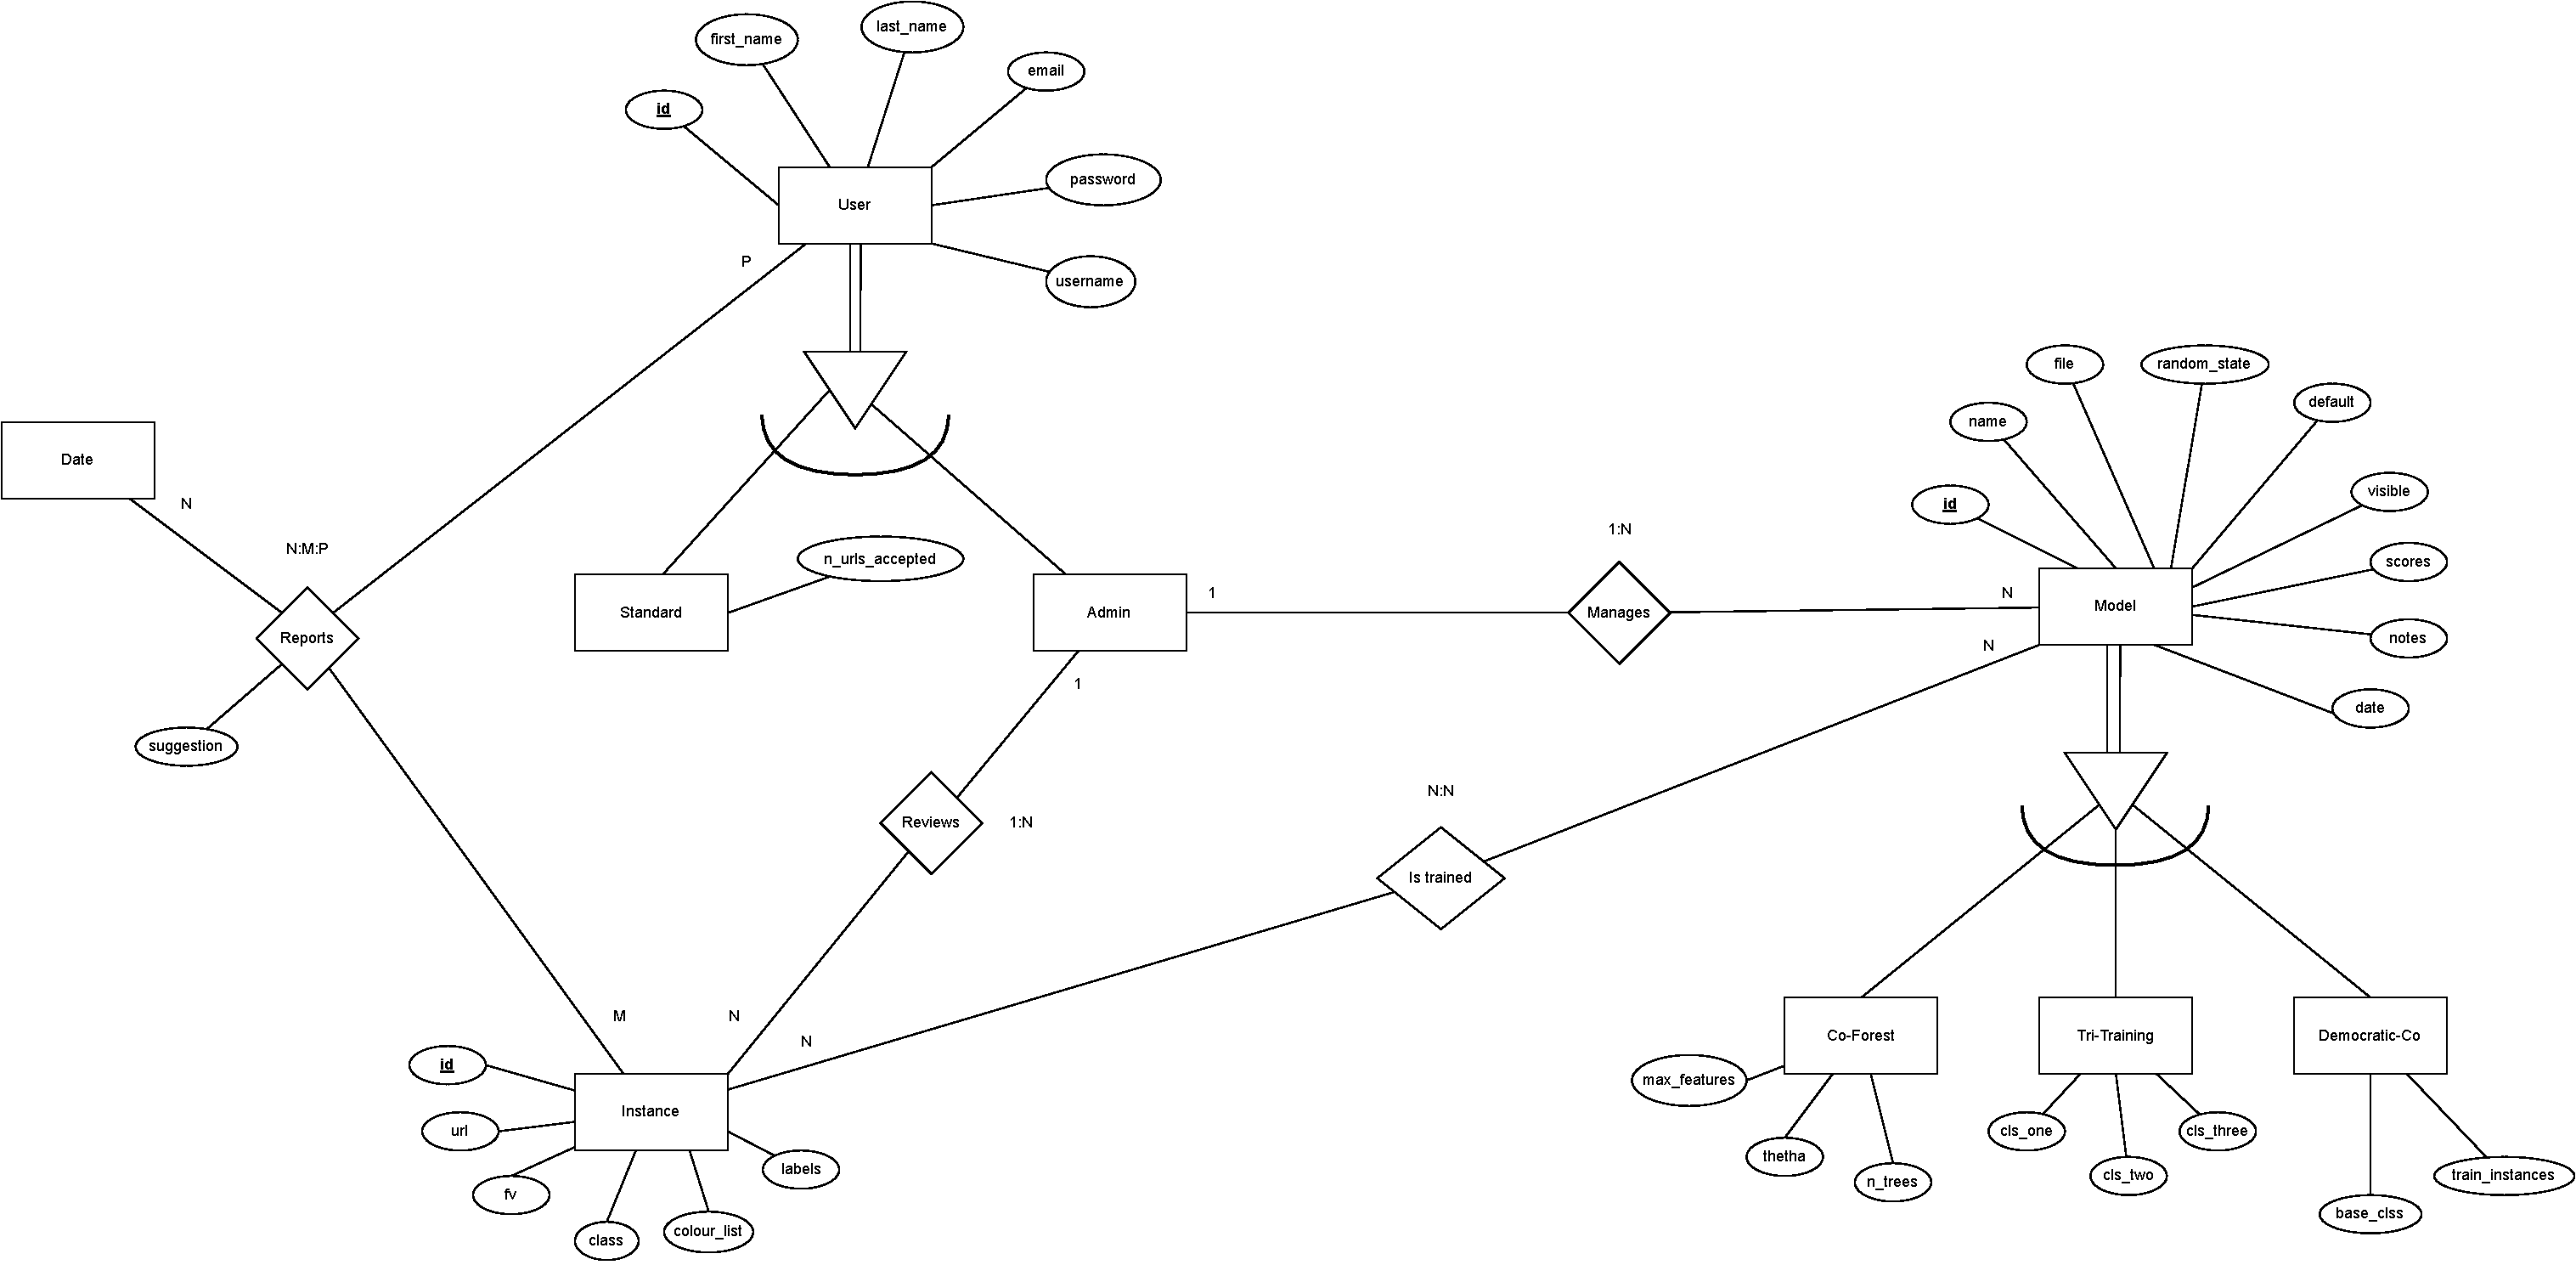
\includegraphics[scale=0.4]{../img/anexos/diagrams/er}
	\label{c:diagrama-er}
\end{figure}
\end{landscape}

\begin{landscape}
	\begin{figure}[h]
		\caption[Diagramas: relacional]{Diagrama relacional de la base de datos}
		\centering
		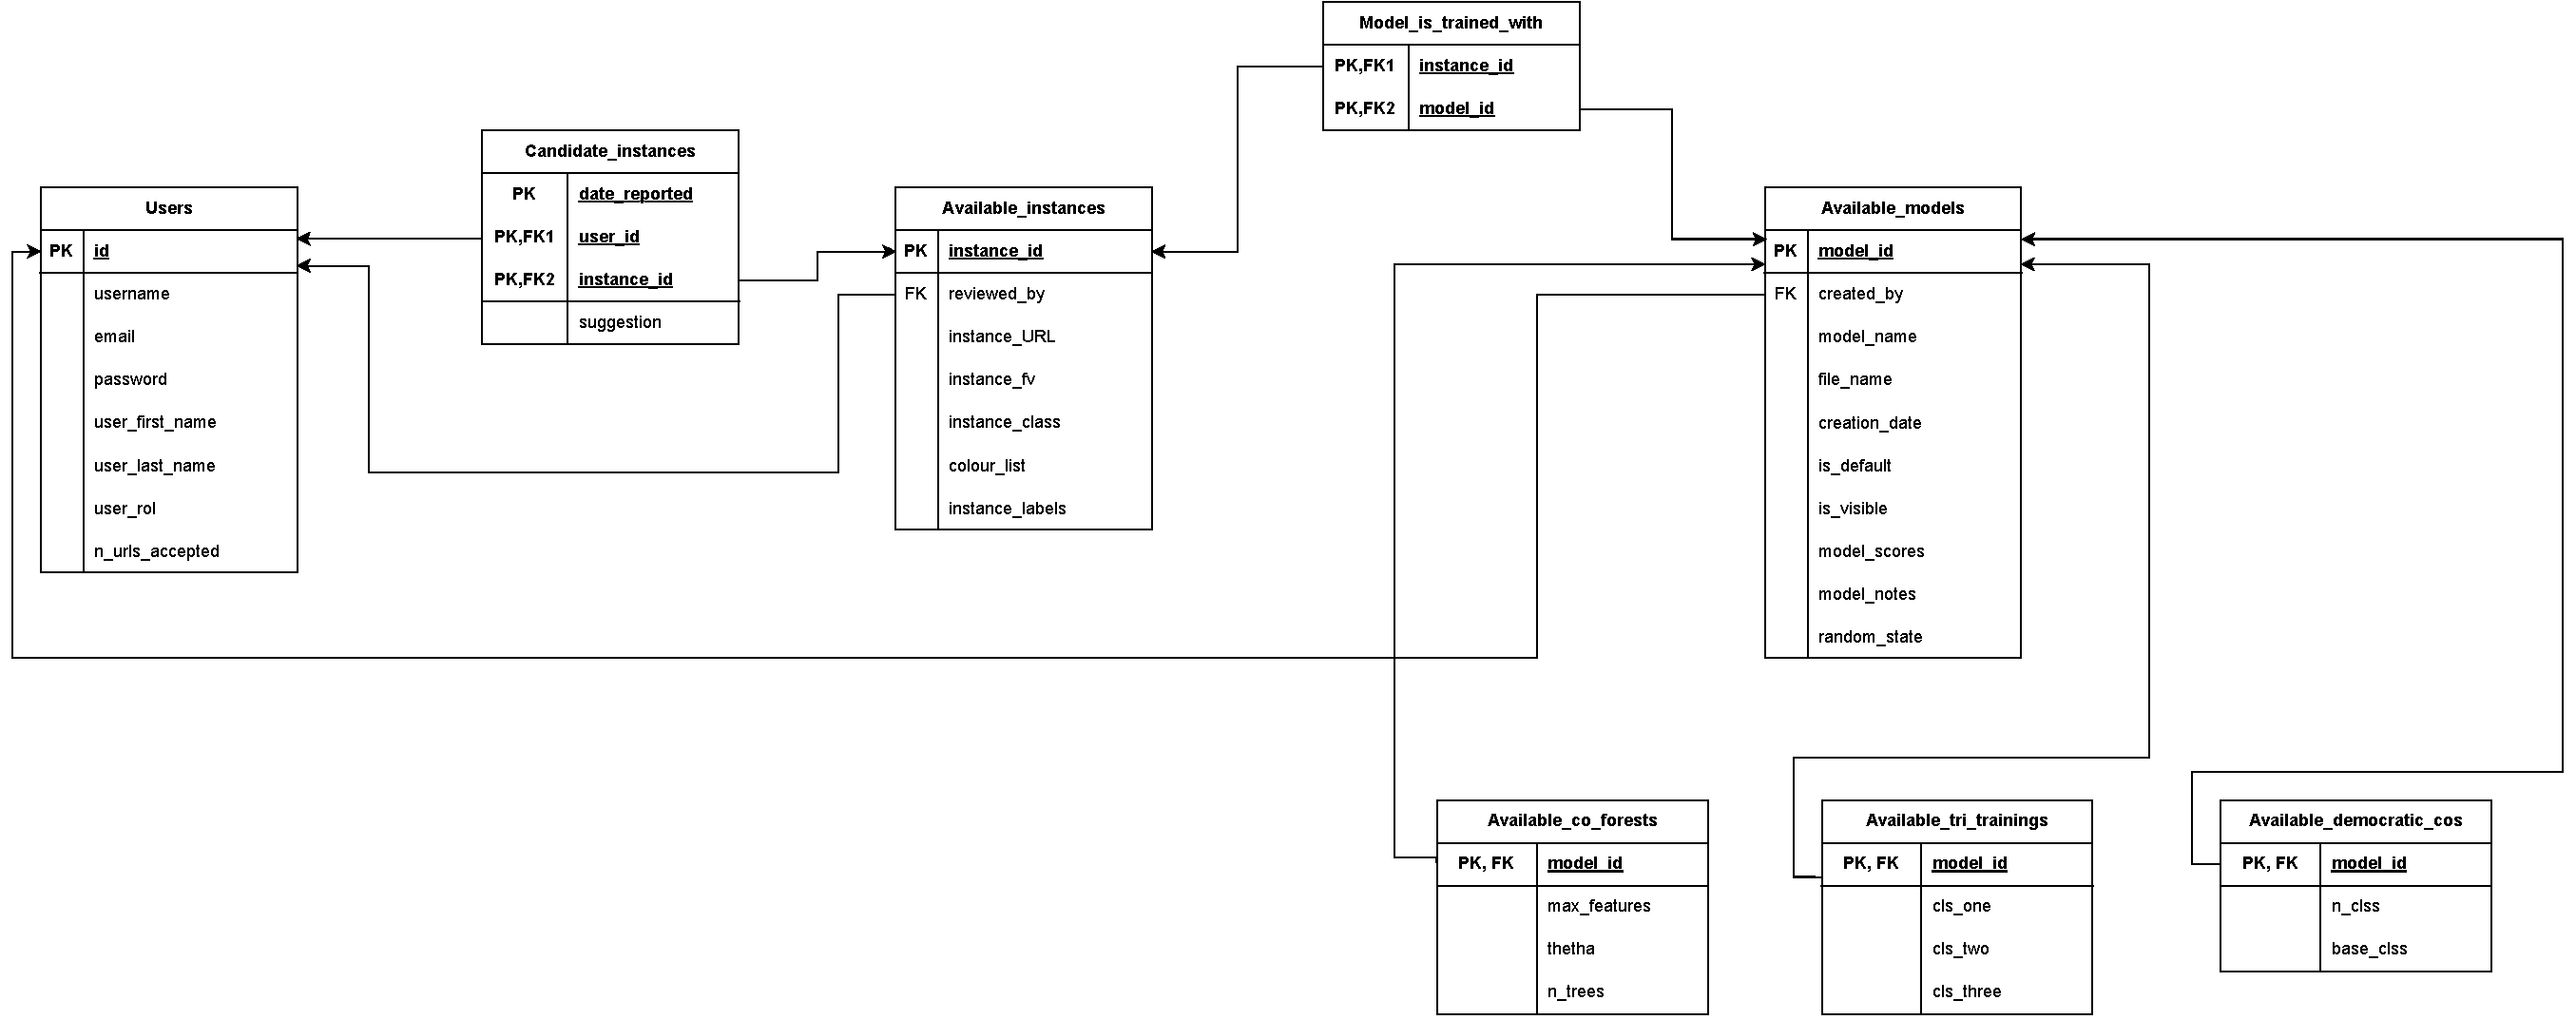
\includegraphics[scale=0.46]{../img/anexos/diagrams/relational}
		\label{c:diagrama-relacional}
	\end{figure}
\end{landscape}

\subsection{Diccionario de datos}

Se adjunta a continuación, para cada tabla, el diccionario de datos correspondiente. \label{c:diccionario_datos}

\subsubsection{Tabla de usuarios (\texttt{Users})}

\begin{table}
	\scalebox{0.80}{
		\begin{tabular}{@{}p{5em} p{6em} p{6em} p{20em}@{}}
			\toprule
			\textbf{Nombre} & \textbf{Tipo} & \textbf{Columna} & \textbf{Descripción}\\
			\midrule
			\texttt{\textbf{\underline{id}}} & \texttt{INTEGER} & \texttt{\textbf{\underline{PK}}} & Identificador. Generado automáticamente mediante una secuencia. \\
			\texttt{username} &  \texttt{VARCHAR(32)} & \texttt{UNIQUE NOT NULL} & Inmutable. Nombre de usuario proporcionado en el registro.\\
			\texttt{email} & \texttt{VARCHAR(256)} & \texttt{UNIQUE NOT NULL} & Inmutable. Email del usuario proporcionado en el registro.\\
			\texttt{password} &  \texttt{BYTEA} & \texttt{NOT NULL} & Contraseña cifrada mediante \texttt{sha-512}. La \textit{salt} se obtiene aleatoriamente y está cifrada en \texttt{sha-256}.\\
			\texttt{user\_first \_name} & \texttt{VARCHAR(64)} & & Nombre del usuario.\\
			\texttt{user\_last \_name} & \texttt{VARCHAR(64)} & & Apellidos del usuario. \\
			\texttt{user\_rol} & \texttt{VARCHAR(8)} & \texttt{NOT NULL} & Rol del usuario. Puede ser <<standard>> o <<admin>>. Por defecto: <<standard>>. \\
			\texttt{n\_urls \_accepted} & \texttt{INTEGER} &  &  Atributo de usuarios <<standard>>. Contador de aquellas instancias que han sido reportadas y aceptadas por un administrador. \\
			\bottomrule
		\end{tabular}
	}
	\caption[Diccionario de datos: Users]{Diccionario de datos. Tabla correspondiente a la clase \texttt{Users}.}
	\label{datadic:users}
\end{table}

La tabla~\ref{datadic:users} almacena la información relevante de cada usuario registrado en la base de datos. Si se comprueba el diagrama E-R, se puede comprobar que una peculiaridad de esta tabla es que es una ISA. Debido a que, además del discriminante (usuario administrador o estándar), únicamente hay un atributo que diferencia ambas clases, se ha decidido implementar utilizando una sola tabla. Cabe destacar que la contraseña está correctamente cifrada mediante  cifrada mediante \texttt{sha-512} y la sal\footnote{\textit{Salt} es un término que se refiere a bits aleatorios usados como entrada (junto a la contraseña) en una función derivadora de claves (cuya salida es la contraseña cifrada).} se ha cifrado en \texttt{sha-256}.


\subsubsection{Tabla de instancias (\texttt{Available\_instances})}

\begin{table}
	\scalebox{0.80}{
	\begin{tabular}{@{}p{6em} p{6em} p{5em} p{20em}@{}}
		\toprule
		\textbf{Nombre} & \textbf{Tipo} & \textbf{Columna} & \textbf{Descripción}\\
		\midrule
			\texttt{\textbf{\underline{instance\_id}}} & \texttt{INTEGER} & \texttt{\textbf{\underline{PK}}} & Identificador. Generado automáticamente mediante una secuencia. \\
			\texttt{reviewed\_by} & \texttt{INTEGER} & \texttt{FK(Users)} & En caso de estar vacío, significa que la URL todavía no ha sido aprobada por un administrador y está en proceso de revisión, por lo que no se puede utilizar para entrenar modelos.\\
			\texttt{instance\_url} & \texttt{VARCHAR(256)} & \texttt{UNIQUE NOT NULL} &  URL de la instancia. Inmutable.\\
			\texttt{instance\_fv} &  \texttt{INTEGER ARRAY[19]} & & Vector de características de la URL.   \\
			\texttt{instance \_class} & \texttt{INTEGER} & & Etiqueta de la clase. Puede valer $0$ si la URL es legítima o $1$ en caso de que sea \textit{phishing}. \\
			\texttt{colour\_list} & \texttt{VARCHAR(12)} & & Puede ser <<black-list>>, <<white-list>> o estar vacío. En caso de contener un valor ha de ser aprobada por un administrador. \\
			\texttt{instance \_labels} & \texttt{CHAR(128)} & &  Se preve que el campo varíe bastante, por lo que el tipo de dato no se ha definido como \texttt{VARCHAR}. Contiene etiquetas relacionadas con la instancia.\\
			\bottomrule
		\end{tabular}
	}
	\caption[Diccionario de datos: Available\_instances]{Diccionario de datos. Tabla correspondiente a la clase \texttt{Available\_instances}.}
	\label{datadic:instances}
\end{table}

La tabla~\ref{datadic:instances} almacena la información asociada a cada instancia disponible en el \textit{dataset}. Las instancias son URLs que pueden ser utilizadas posteriormente para entrenar y probar modelos. Además, esta tabla también almacena enlaces reportados por usuarios por pertenecer a una lista blanca o negra.

\subsubsection{Tabla de modelos (\texttt{Available\_models})}

La tabla~\ref{datadic:models} almacena los modelos de aprendizaje que han sido creados por un administrador y están disponibles en la \textit{web} para su uso.

\begin{table}
	\scalebox{0.80}{
	\begin{tabular}{@{}p{6em} p{6em} p{5em} p{20em}@{}}
		\toprule
		\textbf{Nombre} & \textbf{Tipo} & \textbf{Columna} & \textbf{Descripción}\\
		\midrule
			\texttt{\textbf{\underline{model\_id}}} & \texttt{INTEGER} & \texttt{\textbf{\underline{PK}}} & Identificador. Generado automáticamente mediante una secuencia. \\
			\texttt{created\_by} & \texttt{INTEGER} & \texttt{FK(Users) NOT NULL} &  Enlace al administrador que ha creado un determinado modelo. Dependencia por existencia.\\
			\texttt{model\_name} & \texttt{VARCHAR(32)} & \texttt{UNIQUE NOT NULL} & Inmutable. Nombre común y visible para los usuarios. \\
			\texttt{file\_name} & \texttt{VARCHAR(32)} & \texttt{UNIQUE NOT NULL} & Inmutable. Preferiblemente seguirá la sintáxis \texttt{nombre\_v-a-b-c.pkl}, donde $a$, $b$, $c$ son los números de versión (ejemplo: \texttt{cof\_v-1-0-0.pkl})    \\
			\texttt{creation \_date} & \texttt{TIMESTAMP} & &  Fecha de creación.   \\
			\texttt{is\_default} & \texttt{BOOLEAN} & \texttt{NOT NULL} & Por defecto <<false>>. Determina si un clasificador es el utilizado por defecto (cuando un usuario realiza una consulta y no selecciona ningún modelo).   \\
			\texttt{is\_visible} & \texttt{BOOLEAN} & \texttt{NOT NULL} & Por defecto <<true>>. Determina si un clasificador está visible en la \textit{web} y disponible para ser utilizado.\\
			\texttt{model\_scores} & \texttt{FLOAT(3) ARRAY} & \texttt{NOT NULL} & Por defecto \texttt{[0.0, 0.0, 0.0, 0.0, 0.0]}. Son las últimas estadísticas del último \textit{test} realizado al clasificador. Las columnas (en este orden) corresponden a las métricas \textit{accuracy}, \textit{precision}, \textit{recall}, F1 y ROC AUC. \\			
			\texttt{model\_notes} & \texttt{VARCHAR(128)} & & Notas acerca de los clasificadores base utilizados para crear el \textit{ensemble}. No debería cambiar de valor.\\
			\texttt{random\_state} & \texttt{INTEGER} & & Semilla aleatoria.  \\
			\bottomrule
		\end{tabular}
	}
	\caption[Diccionario de datos: Available\_models]{Diccionario de datos: tabla correspondiente a la clase \texttt{Available\_models}.}
	\label{datadic:models}
\end{table}

Si se comprueba el diagrama E-R, se puede comprobar que esta tabla es una ISA. En este caso se ha decidido implementar considerando que es una interrelación 1:1. Por ello, se ha creado una tabla para la generalización y otra tabla para cada una de las especializaciones. Estas se enumeran a continuación:

\begin{itemize}
	\item \textbf{\texttt{Available\_co\_forests}}: los modelos pertenecientes a este algoritmo poseen los atributos de la tabla~\ref{datadic:coforest}.

	\begin{table}
	\scalebox{0.80}{
	\begin{tabular}{@{}p{6em} p{5em} p{6em} p{20em}@{}}
		\toprule
		\textbf{Nombre} & \textbf{Tipo} & \textbf{Columna} & \textbf{Descripción}\\
		\midrule
				\texttt{\textbf{\underline{model\_id}}} & \texttt{INTEGER} & \texttt{\textbf{\underline{PK}}, FK(Available \_models)} & Identificador. Generado por la secuencia de la tabla padre e introducido mediante código (debe coincidir). \\
				\texttt{max\_features} & \texttt{VARCHAR(4)} & \texttt{NOT NULL} & Parámetro del árbol de decisión. Puede ser <<sqrt>> o <<log2>>. Por defecto <<log2>>.   \\
				\texttt{thetha} & \texttt{FLOAT(3)} & \texttt{NOT NULL} & Parámetro thetha del \textit{ensemble} (umbral de confianza). Por defecto 0.75.   \\
				\texttt{n\_trees} & \texttt{INTEGER} & \texttt{NOT NULL} & Número de árboles. Por defecto 3.   \\
				\bottomrule
			\end{tabular}
		}
		\caption[Diccionario de datos: Available\_co\_forests]{Diccionario de datos: tabla correspondiente a la clase \texttt{Available\_co\_forests}.}
		\label{datadic:coforest}
	\end{table}

	\item \textbf{\texttt{Available\_tri\_trainings}}: los modelos pertenecientes a este algoritmo poseen los atributos de la tabla~\ref{datadic:tritraining}.

	\begin{table}
	\scalebox{0.80}{
	\begin{tabular}{@{}p{6em} p{5em} p{6em} p{20em}@{}}		
		\toprule
		\textbf{Nombre} & \textbf{Tipo} & \textbf{Columna} & \textbf{Descripción}\\
		\midrule
				\texttt{\textbf{\underline{model\_id}}} & \texttt{INTEGER} & \texttt{\textbf{\underline{PK}}, FK(Available \_models)} & Identificador. Generado por la secuencia de la tabla padre e introducido mediante código (debe coincidir).\\
				\texttt{cls\_one} & \texttt{VARCHAR(4)} & \texttt{NOT NULL}  &  Algoritmo del primer estimador base. Puede ser <<kNN>>, <<NB>> o <<tree>>.\\
				\texttt{cls\_two} & \texttt{VARCHAR(4)} & \texttt{NOT NULL} & Algoritmo del segundo estimador base. Puede ser <<kNN>>, <<NB>> o <<tree>>.\\
				\texttt{cls\_three} & \texttt{VARCHAR(4)} & \texttt{NOT NULL} & Algoritmo del tercer estimador base. Puede ser <<kNN>>, <<NB>> o <<tree>>.\\
				\bottomrule
			\end{tabular}
		}
		\caption[Diccionario de datos: Available\_tri\_trainings]{Diccionario de datos: tabla correspondiente a la clase \texttt{Available\_tri\_trainings}.}
		\label{datadic:tritraining}
	\end{table}

	\item \textbf{\texttt{Available\_democratic\_cos}}: los modelos pertenecientes a este algoritmo poseen los atributos de la tabla~\ref{datadic:democraticco}.

	\begin{table}
	\scalebox{0.80}{
	\begin{tabular}{@{}p{6em} p{5em} p{6em} p{20em}@{}}		
		\toprule
		\textbf{Nombre} & \textbf{Tipo} & \textbf{Columna} & \textbf{Descripción}\\
		\midrule
				\texttt{\textbf{\underline{model\_id}}} & \texttt{INTEGER} & \texttt{\textbf{\underline{PK}}, FK(Available \_models)} & Identificador. Generado por la secuencia de la tabla padre e introducido mediante código (debe coincidir).\\
				\texttt{n\_clss} & \texttt{INTEGER} & \texttt{NOT NULL} & Número de clasificadores base.\\
				\texttt{base\_clss} & \texttt{VARCHAR(4) ARRAY} & \texttt{NOT NULL}  & Array con los algoritmos pertenecientes a los estimadores base. Los valores que puede contener son <<kNN>>, <<NB>> o <<tree>>.\\
				\bottomrule
			\end{tabular}
		}
		\caption[Diccionario de datos: Available\_democratic\_cos]{Diccionario de datos: tabla correspondiente a la clase \texttt{Available\_democratic\_cos}.}
		\label{datadic:democraticco}
	\end{table}
\end{itemize}

\subsubsection{Tablas de relación}

Se enumeran a continuación las tablas que son resultado de una relación entre entidades.

\begin{itemize}
	\item \textbf{\texttt{Candidate\_instances}}: en la tabla~\ref{datadic:candidate_instances} se almacenan aquellas instancias que han sido reportadas por un usuario y necesitan ser revisadas por un administrador antes de ser incluidas en el \textit{dataset} utilizable de la aplicación. Como se puede comprobar, se trata de una relación ternaria entre el usuario, la instancia reportada y la fecha (puede ser que un usuario reporte la misma URL más de una vez en dos fechas distintas). Es destacable que este es uno de los casos (excepción) en los que no merece la pena que la entidad <<Fecha>> pase a ser tabla debido a que no posee ninguna característica relevante.
	
		\begin{table}
		\scalebox{0.80}{
		\begin{tabular}{@{}p{7em} p{6em} p{7em} p{17em}@{}}		
			\toprule
			\textbf{Nombre} & \textbf{Tipo} & \textbf{Columna} & \textbf{Descripción}\\
			\midrule
				\texttt{user\_id} & \texttt{INTEGER} & \texttt{FK(Users)} & Identificador del usuario que ha reportado la URL. \\
				\texttt{instance\_id} & \texttt{INTEGER} & \texttt{FK(Available \_instances)} & Identificador de la URL reportada. \\
				\texttt{date\_reported} & \texttt{TIMESTAMP} & & Fecha de envío del formulario.     \\
				\texttt{suggestion} & \texttt{VARCHAR(16)} & \texttt{NOT NULL} & Lo que el usuario denuncia que la URL es (ejemplo: <<white-list>>).   \\\\
				\multicolumn{3}{l}{\hfill \texttt{\textbf{\underline{PK(user\_id, instance\_id, date\_reported)}}}} & Clave primaria compuesta de la relación. \\
				\bottomrule
			\end{tabular}
		}
		\caption[Diccionario de datos: Candidate\_instances]{Diccionario de datos: tabla correspondiente a la clase \texttt{Candidate\_instances}.}
		\label{datadic:candidate_instances}
		\end{table}

	\item \textbf{\texttt{Model\_is\_trained\_with}}: en la tabla~\ref{datadic:modeltrainedwith} se almacena qué instancia ha sido utilizada para entrenar qué modelo en el sistema.
	
		\begin{table}
		\scalebox{0.80}{
		\begin{tabular}{@{}p{7em} p{6em} p{7em} p{17em}@{}}		
			\toprule
			\textbf{Nombre} & \textbf{Tipo} & \textbf{Columna} & \textbf{Descripción}\\
			\midrule
				\texttt{model\_id} & \texttt{INTEGER} & \texttt{FK(Available \_models)} & Identificador del modelo que ha sido entrenado. \\
				\texttt{instance\_id} & \texttt{INTEGER} & \texttt{FK(Available \_instances)} & Identificador de la instancia utilizada en la fase de entrenamiento. \\\\
				\multicolumn{3}{l}{\hfill \texttt{\textbf{\underline{PK(model\_id, instance\_id)}}}} & Clave primaria compuesta de la relación. \\
				\bottomrule
			\end{tabular}
		}
		\caption[Diccionario de datos: Model\_is\_trained\_with]{Diccionario de datos: tabla correspondiente a la clase \texttt{Model\_is\_trained\_with}.}
		\label{datadic:modeltrainedwith}
	\end{table}
\end{itemize}


\section{Diseño procedimental}
\label{s:diseño-procedimental}

En el desarrollo de \textit{software}, el diseño procedimental se refiere a la definición de pasos ordenados para realizar una determinada funcionalidad. Se utiliza para crear métodos y se basa en la descomposición del problema en pequeñas tareas ejecutadas secuencialmente para alcanzar el resultado deseado. Para ello, se ha hecho uso de diagramas de secuencia. Estos muestran la interacción entre distintos componentes en un sistema.

Con el fin de facilitar la comprensión de ciertos métodos, se muestran a continuación los diagramas de las principales funcionalidades implementadas.

\begin{itemize}
	\item \textbf{Página principal}: en el diagrama~\ref{c:diagrama-seq-index} se representan los pasos seguidos en la página principal. Como se puede comprobar, el usuario realiza una petición y permanece esperando en la pantalla de carga correspondiente. Mientras tanto, el analizador procesa su petición.
	
	Para extraer el vector de características es necesario que la dirección introducida sea alcanzable. En caso de que no lo sea, se realizan correcciones (completar protocolos, corregir sintáxis, etc.). Posteriormente se intenta recuperar posible información existente en la base de datos acerca de dicha instancia (si pertenece a una lista blanca o negra, si ya se tiene almacenado su vector de características, etc.).
	
	Si la dirección no es alcanzable y no hay información previa, se devuelve al usuario un mensaje informativo (es una excepción, no se puede analizar ni mostrar nada).
	
	En el caso de que exista información previa acerca de dicha instancia (el vector de características está almacenado), se puede analizar (ya sea llamable o no). Este camino también es seguido en caso de que el usuario seleccione el <<análisis rápido>>, ya que recuperar el vector de características de la base de datos no es temporalmente costoso.
	
	Por último, en caso de que la URL sea llamable y si no se ha recorrido ningún camino previo, se analiza utilizando el método de extracción de vector de características expuesto en la sección teórica de la memoria. Este proceso requiere unos 40 segundos.
	
	Si no ha ocurrido ninguna excepción, en cualquiera de las opciones se ha extraído el vecto de características. Por lo tanto, sólo queda analizar y mostrar los resultados haciendo uso de técnicas visuales (gráficos interactivos) en el \textit{dashboard}, por lo que se redirige a esta pantalla. En caso de que ocurra alguna excepción, el usuario será devuelto a la página principal con un mensaje informativo.
	
	\begin{landscape}
	\begin{figure}[h]
		\caption[Diagramas: secuencia (página principal)]{Diagrama de secuencia de la página principal del analizador.}
		\centering
		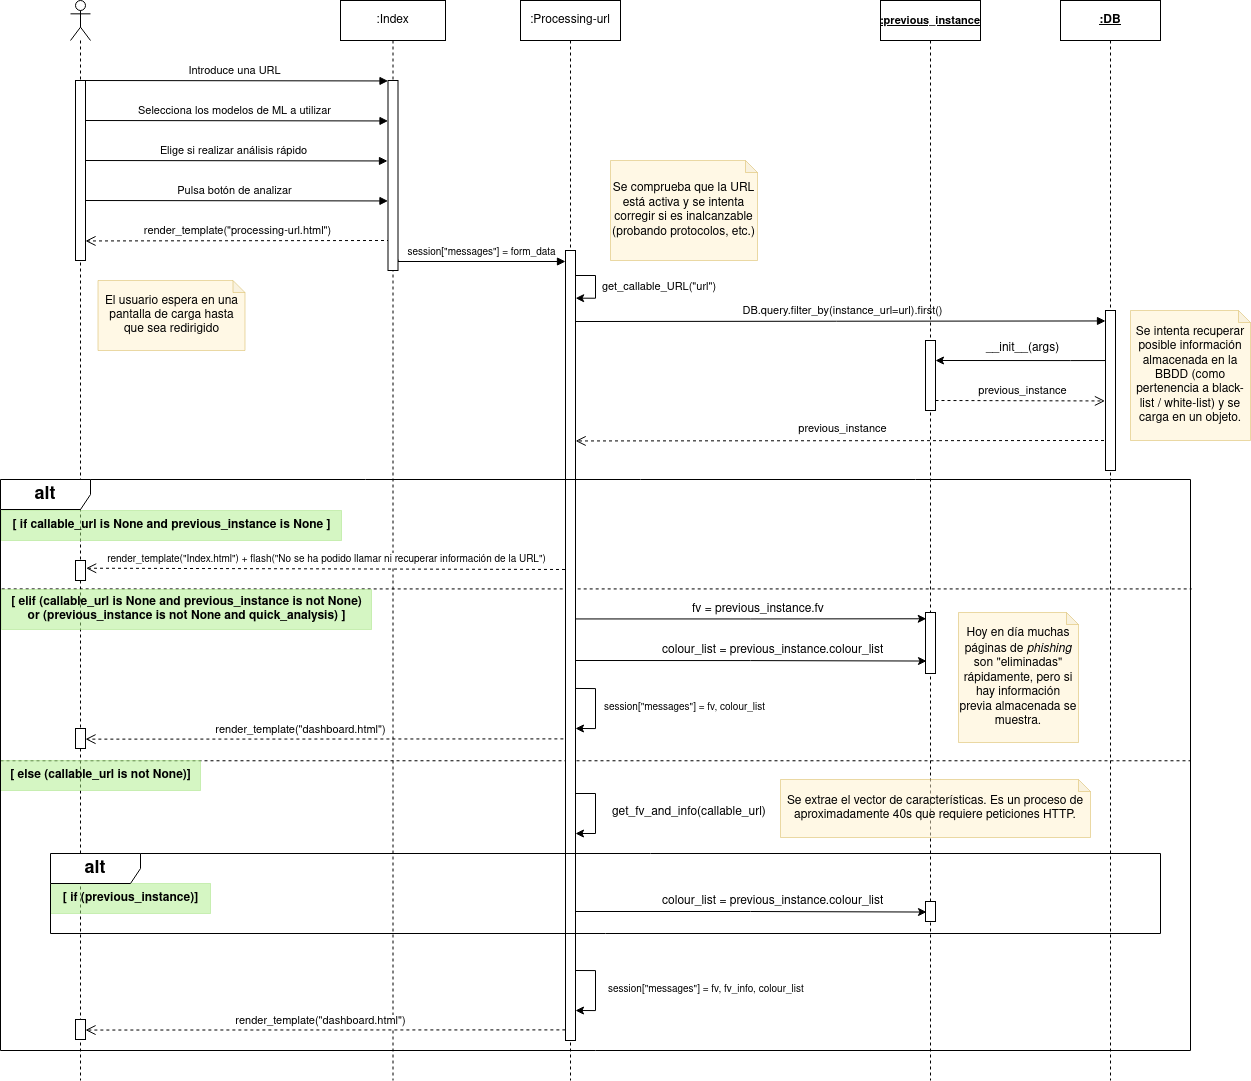
\includegraphics[scale=0.37]{../img/anexos/diagrams/sequence-index}
		\label{c:diagrama-seq-index}
	\end{figure}
	\end{landscape}


	\item \textbf{Página para reportar una URL}: la secuencia se ilustra en el diagrama~\ref{c:diagrama-seq-report_url}. Como se puede comprobar, el usuario tan solo ha de introducir su URL, seleccionar el tipo (lista blanca o lista negra) y aceptar.
	
	Como internamente la tabla donde se almacenan las URLs reportadas necesita información para incluir un nuevo registro (identificador de la instancia y del usuario), se intenta recuperar la instancia que se está reportando. En caso de no existir, se crea una nueva y se añade a la base de datos. Por último, se incluye el reporte con los datos y se redirige al usuario a la misma página con un mensaje informativo.
	
	Es destacable que un usuario registrado no va a poder acceder a esta pantalla (antes será redirigido por el sistema de control a la página de inicio de sesión).
	
	\begin{figure}[h]
		\caption[Diagramas: secuencia (reportar url)]{Diagrama de secuencia de la página para reportar una URL.}
		\centering
		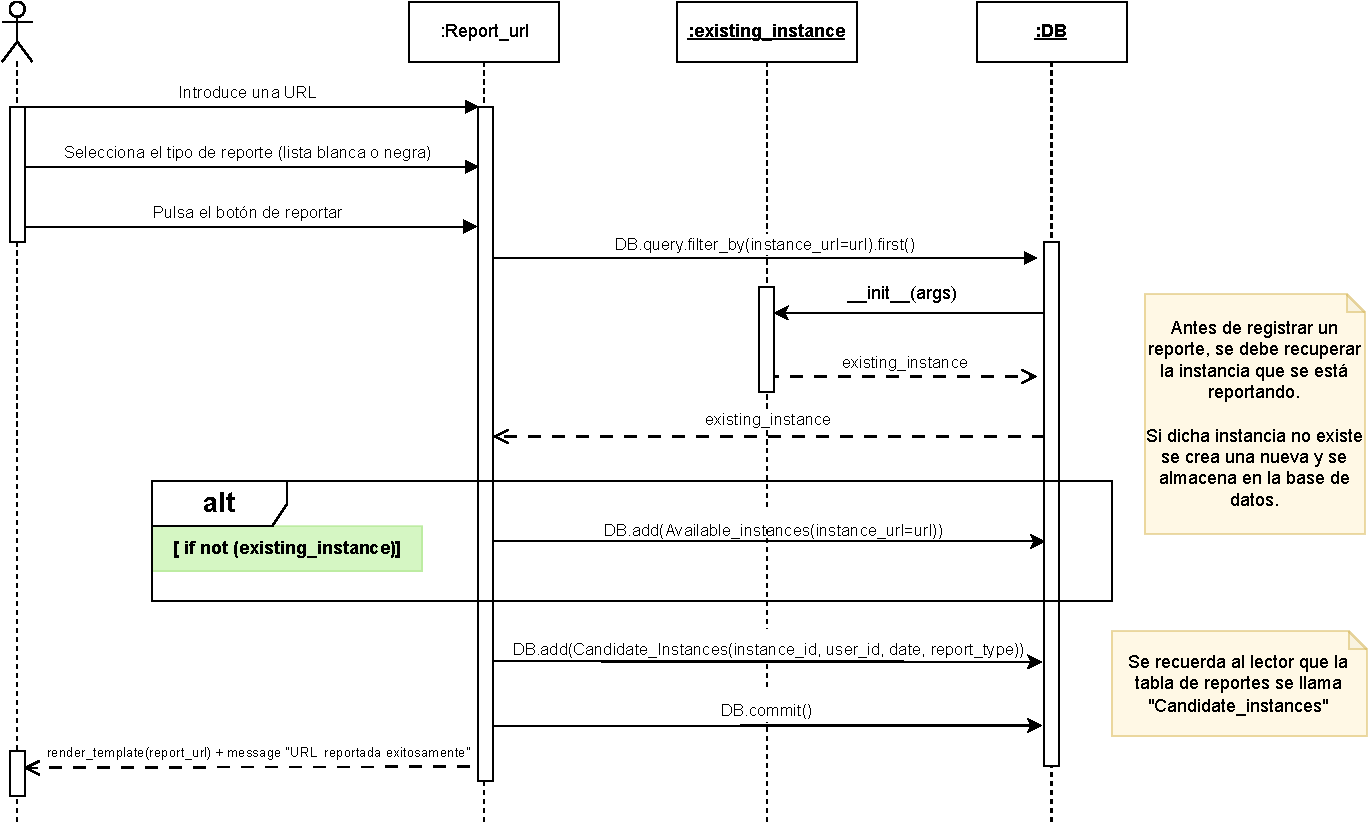
\includegraphics[scale=0.4]{../img/anexos/diagrams/sequence-report_url}
		\label{c:diagrama-seq-report_url}
	\end{figure}


\end{itemize}

\section{Diseño arquitectónico}
\label{s:diseño-arquitectonico}´

